\documentclass[8pt]{beamer}
\usepackage[T1]{fontenc}
\usepackage[francais]{babel}
\usepackage{tikz}
\usetikzlibrary{arrows,shapes}
\usepackage{pslatex}
\usepackage{textcomp}
\usepackage[utf8]{inputenc}
\usepackage{wrapfig}
\usepackage{graphicx}
\usepackage[section]{placeins}
\usepackage{lscape}
\usepackage{float}
\usepackage{amssymb}
\usepackage{wasysym}
\usepackage{pgf}
\usepackage{alltt}
\usepackage{eso-pic}
\usepackage{url}
\usepackage{tikz}
\usepackage{listings}
\usepackage{color}
\definecolor{mymauve}{rgb}{0.58,0,0.82}

\lstset{language=C++,
basicstyle=\footnotesize,
keywordstyle=\color{red}\bfseries,
breaklines=true,
commentstyle=\color{blue},
stringstyle=\color{mymauve},
literate={ô}{{\^o}}1 {é}{{\'e}}1 {à}{{\`a}}1 {è}{{\`e}}1 {î}{{\^{\i}}}1 {ê}{{\^e}}1 {ç}{{\c c}}1,
morekeywords={string,fstream,ofstream,ifstream}
}
\usepackage{hyperref}

%\hypersetup{urlcolor=blue}

\usetheme{CambridgeUS}


\title[DQM4HEP - v04-02-00]{DQM for SDHCAL detector - Status report}
\institute[UCBL - IPNL - UGent]{Université Claude Bernard Lyon 1 - Institut de Physique Nucléaire de Lyon / Ghent University}
\author[Eté - Pingault - Mirabito]{{\bf \large R. \'Eté, A. Pingault, L. Mirabito}}
\date{\today}

\DeclareUnicodeCharacter{00A0}{ }

\setbeamertemplate{itemize items}[ball]
\definecolor{MyGreen}{rgb}{0.1,0.5,0.1}
\setbeamercolor{structure}{fg=red!70!black}
\setbeamercolor{block title}{bg=red!70!black,fg=black}
\addtobeamertemplate{block begin}{\pgfsetfillopacity{0.5}}{\pgfsetfillopacity{1}}

\begin{document}


  %%%%%%%%%%%%%% Page de présentation %%%%%%%%%%%%%%
  \begin{frame}

    \titlepage
    \begin{center}
      
\includegraphics[width=0.5\textwidth]{logo/logo-ucbl-ipnl.jpg} ~~~~~~~~~~~
      
\includegraphics[width=0.2\textwidth]{logo/Ghent_University_logo.png}
    \end{center}
  \end{frame}


  %% OVERVIEW %%
  \section{Framework overview}


  %% GENERAL %%
  \begin{frame}
    \frametitle{\secname}
    \framesubtitle{DQM4HEP : an online monitoring system for data quality}

    \begin{block}{Key points}
      \begin{itemize}
        \item Event and histogram distributed system : server/client paradigm
        \item Set of interfaces for data analysis, adapted to DQM purpose
        \item Visualization interface (Qt GUI)
        \item Large scale remote process management
        \item Generic IO support for any edm (opt. LCIO)
        \item Full size HEP experiment to single detector prototype design
        \item Interface to generic online event buidler (levbdim)
        \item ELog interface
      \end{itemize}
    \end{block}
    ~ \\
    Set of interfaces inspired from CMS DQM system (monitor elements, collectors). \\
    ~ \\
    Application flow inspired from ALICE DQM system, AMORE (cycles).

  \end{frame}


  %% PACKAGES %%
  \begin{frame}
    \frametitle{\secname}
    \framesubtitle{DQM4HEP packages}
    One location : \href{https://github.com/DQM4HEP}{\tt https://github.com/DQM4HEP} \\
    Webpage : \href{dqm4hep.github.io}{\tt dqm4hep.github.io} \\
    \begin{block}{The main package : DQM4HEP}
      Installation package for sub-packages (CMake). \\
      Sub-packages :
      \begin{itemize}
        \item \textbf{dim} : Distributed Information Management (Delphi). Manage client/server communications
        \item \textbf{dimjc} : DIM Job Control (L. Mirabito). Remote process management using dim.
        \item \textbf{levbdim} : DIM online event builder (L. Mirabito). Generic online multi-detector event builder
        \item \textbf{jsoncpp} : Json I/O for dimjc ad levbdim
        \item \textbf{log4cxx} : logging library (use apt-get)
        \item \textbf{DQMCore} : Core part of the DQM system. Client/server interfaces, analysis, IO, run control interface, plugin management ...
        \item \textbf{DQMViz} : Qt visualization interfaces. Job control gui client, monitoring gui client, run control server gui (standalone).
        \item \textbf{xdrstream} : Generic Xdr serializer
        \item \textbf{xdrlcio} : Lcio serialization using xdrstream (buffer -> socket)
        \item \textbf{DQM4ILC} : ILC specific implementation (marlin helper, lcio streamer, lcio file service, etc ...)
      \end{itemize}
    \end{block}
  \end{frame}


  %% Workflow %%
  \begin{frame}
    \frametitle{\secname}
    \framesubtitle{DQM4HEP workflow}
    \begin{center}
      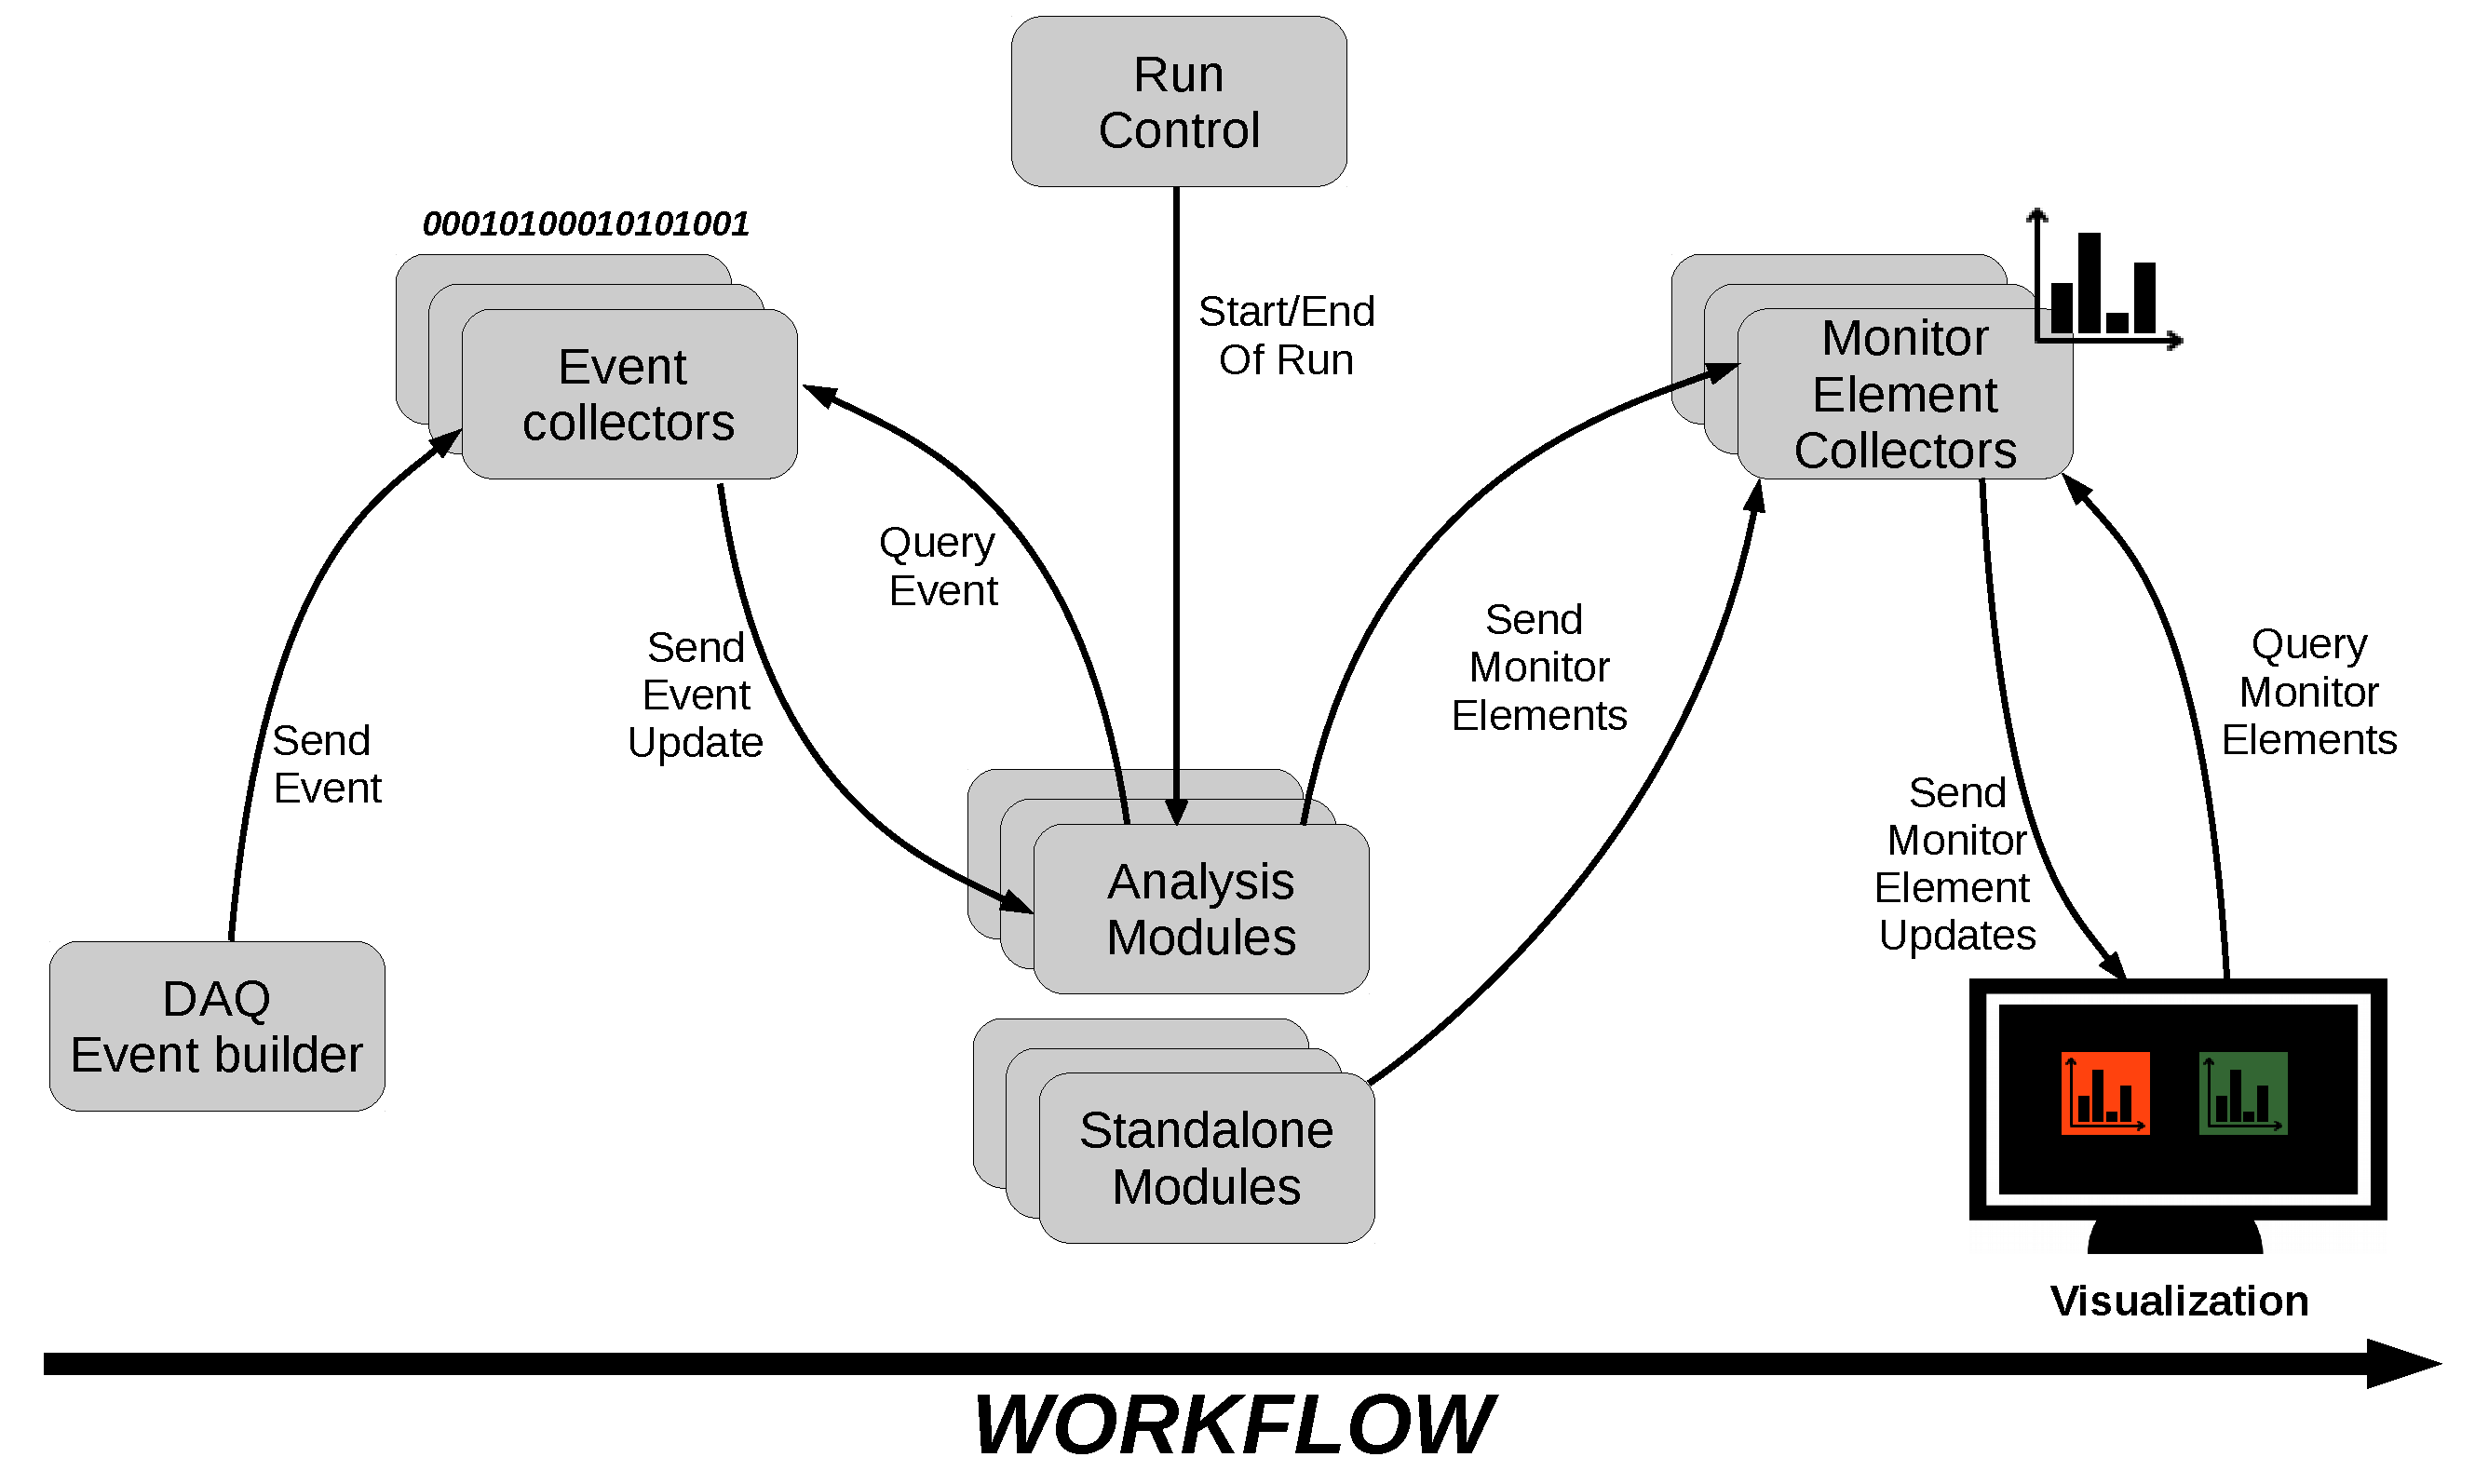
\includegraphics[width=\textwidth]{figs/DQM4HEP_workflow.pdf}
    \end{center}
  \end{frame}
  
  
  
    \begin{frame}[containsverbatim]
    \frametitle{\secname}
    \framesubtitle{Online builder interface}
  
      New package (optionnal) in DQM4HEP : levbdim \\
      Use \verb|-DBUILD_EVB=ON| cmake flag to compile levbdim support \\
      ~ \\
      Generic online event builder based on DIM 
      \begin{itemize}
        \item Uses DIM sockets to collect raw data from different source and dump them in shared memory
        \item Groups all data packets into buffer list by reading them into shared memory
        \item Pass them to user callback functions
      \end{itemize}
      ~ \\      
      Developed by the SDHCAL team for future combined test beams with ECAL. \\
      Can managed many subdetectors (ECAL, HCAL, Cherenkov, TPC, ...) \\
      ~ \\
      Interface implemented in DQMCore to feed the DQM system with raw data. \\
      Application provided and use plugin manager to get user raw data converters to event interface
    
  \end{frame}
  
  
  \begin{frame}[containsverbatim]
    \frametitle{\secname}
    \framesubtitle{Online builder interface}
  
    \begin{center}
      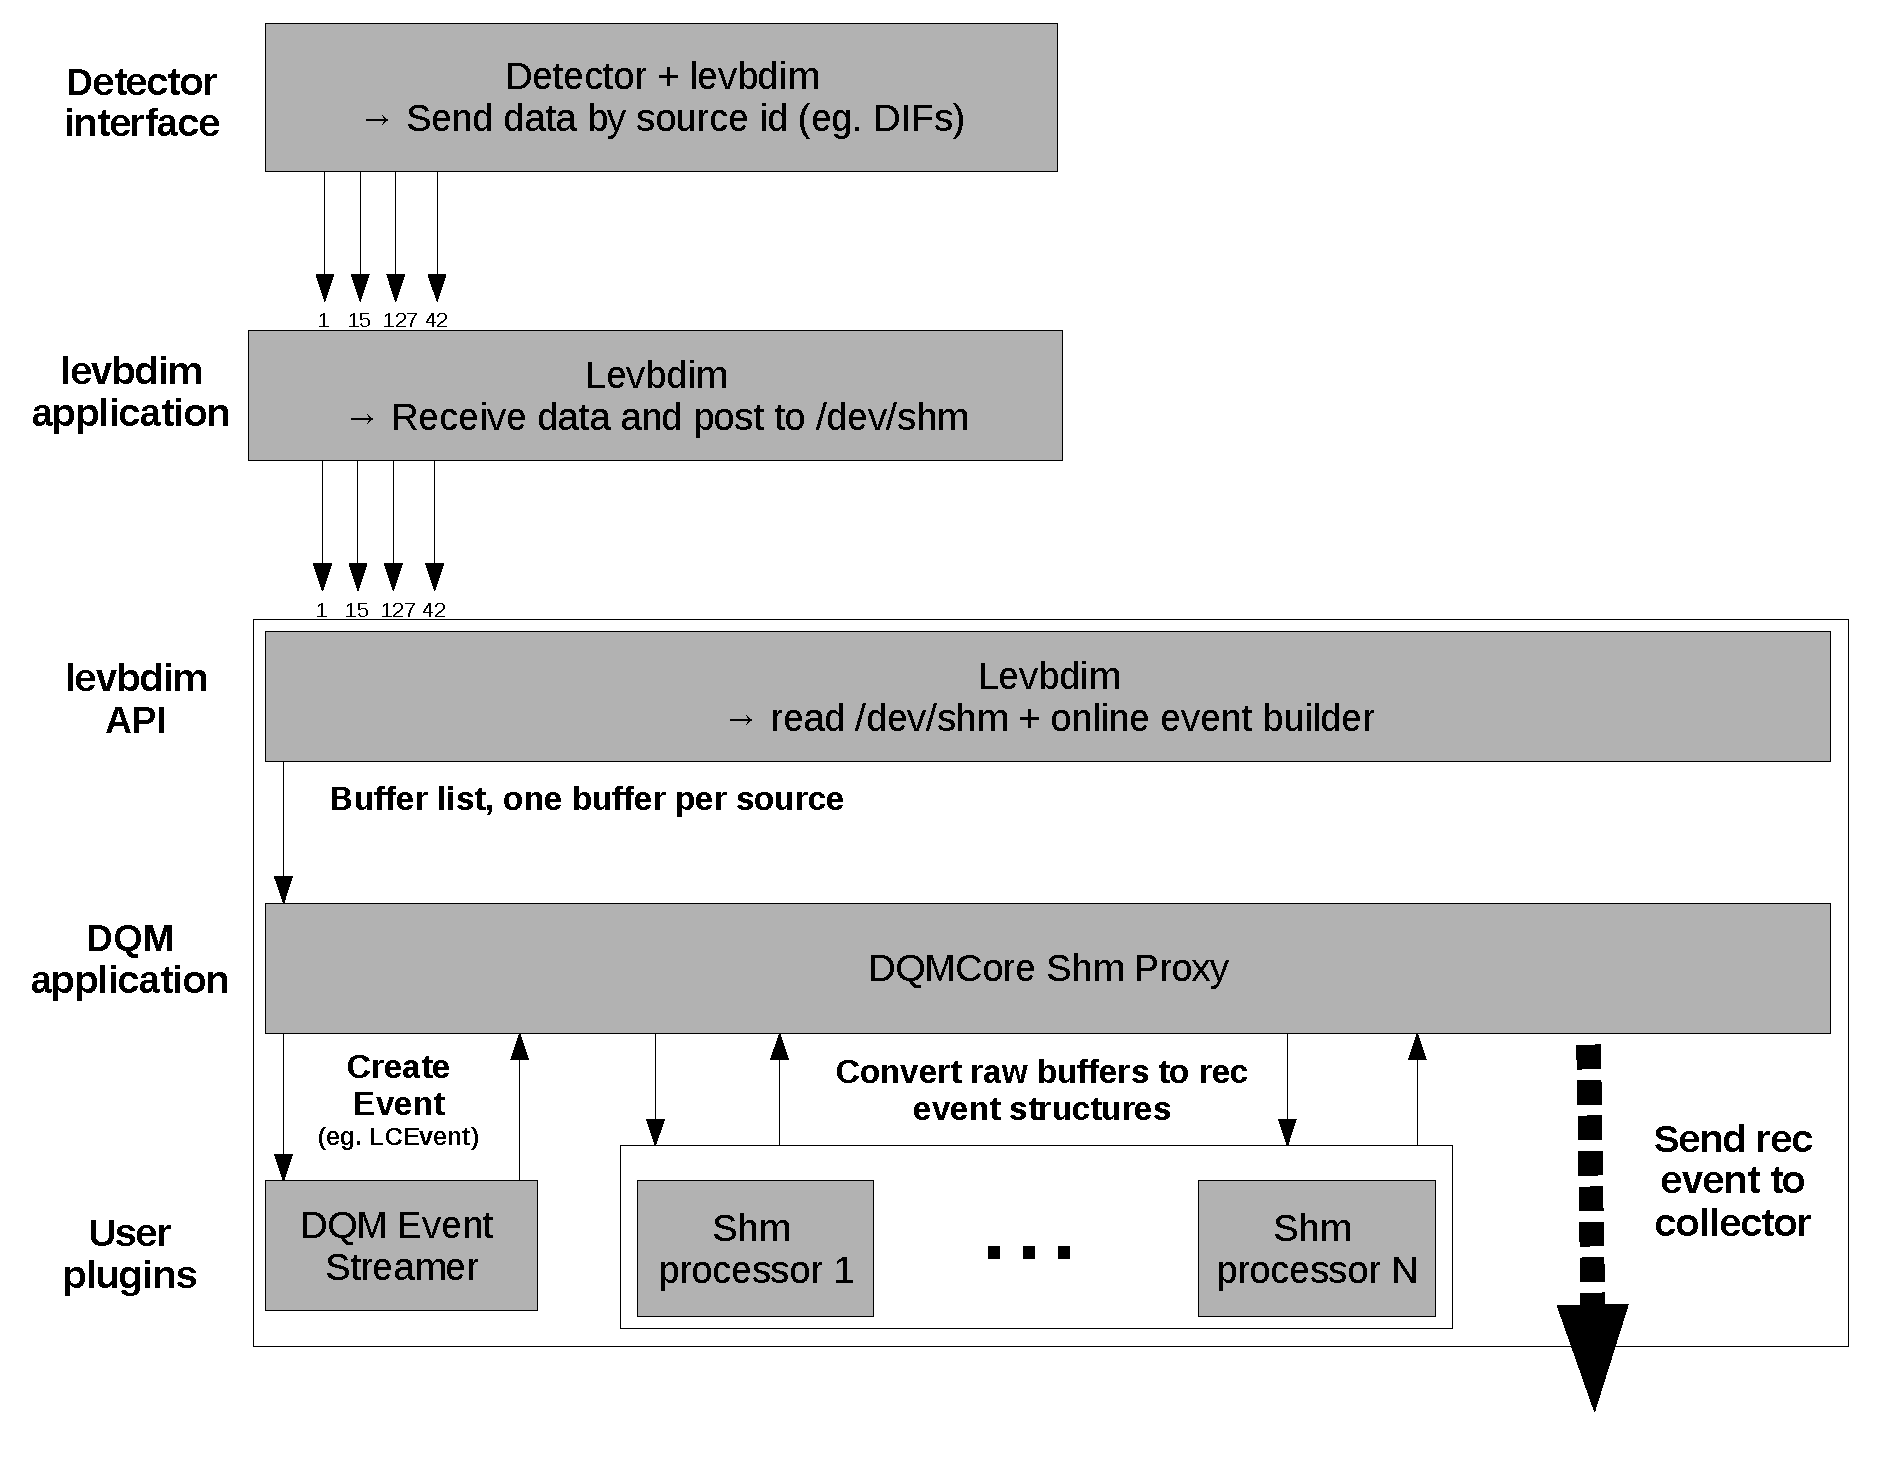
\includegraphics[width=0.8\textwidth]{figs/DQMeventbuilder.pdf}
    \end{center}
    
  \end{frame} 
  


  %% MODULE APPLICATION %%
  \begin{frame}[containsverbatim]
    \frametitle{\secname}
    \framesubtitle{Module applications - analysis module}

    \begin{minipage}{0.78\textwidth}
      \begin{block}{Purpose}
        \begin{itemize}
          \item Receive online events from a collector server and process them
          \item Produce monitor elements (histograms, scalars, generic TObject)
          \item Follow the run control signals (SOR, EOR)
        \end{itemize}
      \end{block}

      \begin{itemize}
        \item \textbf{Init} : Initialize the application : load dlls, declare services, etc ... Wait for a SOR
        \item \textbf{Start of run} : start cycles loop, open archive
        \item \textbf{Start of cycle} : start a cycle of '\textit{process event}'
        \item \textbf{Process event} : Process incoming event, fill monitor elements, etc ...
        \item \textbf{End of cycle} : send subscribed monitor elements, update archive (opt).
        \item \textbf{End of run} : Wait for SOR, close archive (opt).
        \item \textbf{End} : Clean and exit module.
      \end{itemize}
      Helpers to evaluate data quality : \verb|DQMQualityTest| (ie. Kolmogorov or $\chi^2$ test) \\
      Quality test results sent together with the monitor elements to the collector \\
      ~ \\
      To implement online DQM analysis, user must implement the \verb|DQMAnalysisModule| interface. A shared library must be build and loaded in the application using the plugin system (\verb|export DQM4HEP_PLUGIN_DLL=libMyModule.so|). \\

    \end{minipage}
    \begin{minipage}{0.2\textwidth}
      \begin{flushright}
        \begin{tikzpicture}[scale=0.8]
        \node[draw] (I) at (0,-1) {Init};
        \node[draw] (SR) at (0,-2) {Start of run};
        \node[draw] (SC) at (0,-3) {Start of cycle};
        \node[draw] (PE) at (0,-4) {Process event};
        \node[draw] (EC) at (0,-5) {End of cycle};
        \node[draw] (ER) at (0,-6) {End of run};
        \node[draw] (E) at (0,-7) {End};
        \tikzset{fleche/.style={->,>=latex,thick}}
        \draw[fleche] (0,0) node {$\bullet$} -- (I);
        \draw[fleche] (I) -- (SR);
        \draw[fleche] (SR) -- (SC);
        \draw[fleche] (SC) -- (PE);
        \draw[fleche] (PE) -- (EC);
        \draw[fleche] (EC) -- (ER);
        \draw[fleche] (ER) -- (E);
        \draw[fleche] (E) -- (0,-8) node {$\bullet$};
        \draw[fleche] (0,-4.5) -- (1.3,-4.5) -- (1.3,-3.5) -- (0,-3.5);
        \draw[fleche] (0,-5.5) -- (1.4,-5.5) -- (1.4,-2.5) -- (0,-2.5);
        \draw[fleche] (0,-6.5) -- (1.5,-6.5) -- (1.5,-1.5) -- (0,-1.5);
        \end{tikzpicture}\\
        Analysis module~~~~\\ application flow~~~~~
      \end{flushright}
    \end{minipage}
  \end{frame}


  \begin{frame}
    \frametitle{\secname}
    \framesubtitle{Gui visualisation}

	  Gui interfaces for DQM client developed :

      \begin{itemize}
        \item Run control, job control, online monitoring
        \item Written with Qt4 framework     
\includegraphics[width=.03\textwidth]{logo/Qt_CMYK_color}
        \item Easily configurable with json and xml.
      \end{itemize}

      \end{frame}


 %% Run Control %%
 \begin{frame}
    \frametitle{\secname}
    \framesubtitle{ Run Control GUI }
    \begin{center}
      \begin{overlayarea}{\textwidth}{\textheight}
        \begin{columns}
      	\column{.3\textwidth}
	      \vspace{-2em}
          \begin{center}
            \begin{onlyenv}<1>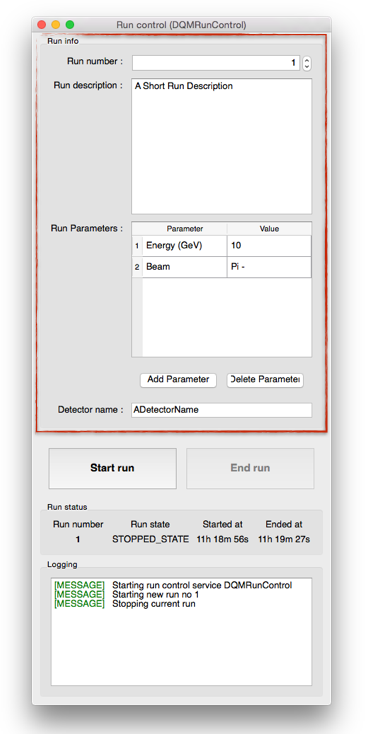
\includegraphics[width=\textwidth]{figs/RunControl/RunControl_Infos.png}\end{onlyenv}
            \begin{onlyenv}<2>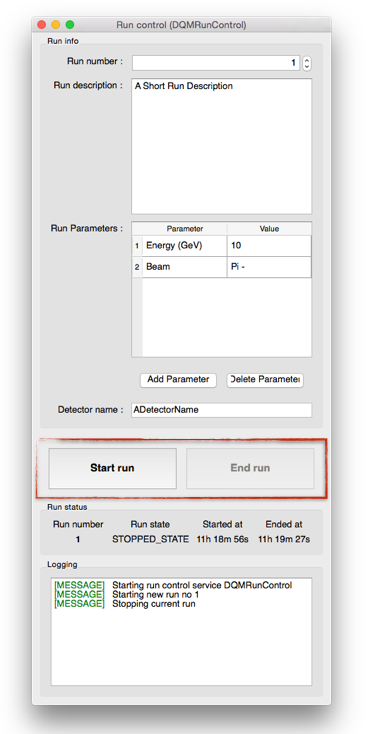
\includegraphics[width=\textwidth]{figs/RunControl/RunControl_SOR.png}\end{onlyenv}
            \begin{onlyenv}<3>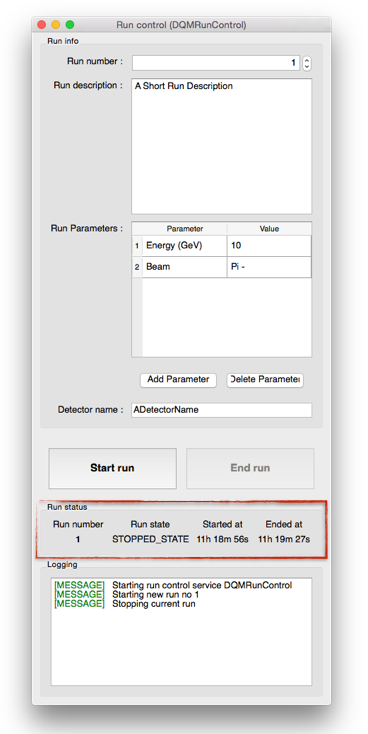
\includegraphics[width=\textwidth]{figs/RunControl/RunControl_Status.png}\end{onlyenv}
            \begin{onlyenv}<4>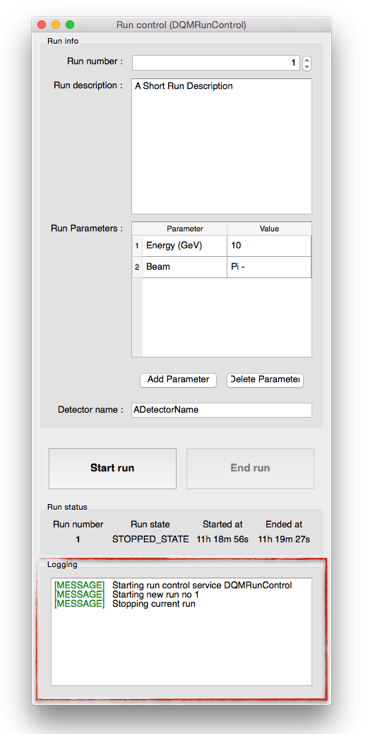
\includegraphics[width=\textwidth]{figs/RunControl/RunControl_logging.png}\end{onlyenv}
          \end{center}
      	  \column{.7\textwidth}
          \begin{itemize}
            \uncover<1->{\item Parametrisation of run with run number, detector name, run description and parameters }
         	  \uncover<1->{\item Send SOR and EOR signals }
         	  \uncover<1->{\item Control run status ( State, Started/Stopped time ) }
         	  \uncover<1->{\item Every action is logged for easy information overview }
          \end{itemize}
        \end{columns}
      \end{overlayarea}
    \end{center}
  \end{frame}


 %% Job Interface %%
  \begin{frame}
    \frametitle{\secname}
    \framesubtitle{ Job Control GUI }

      \begin{overlayarea}{\textwidth}{\textheight}
      	\begin{center}
        		\begin{onlyenv}<5>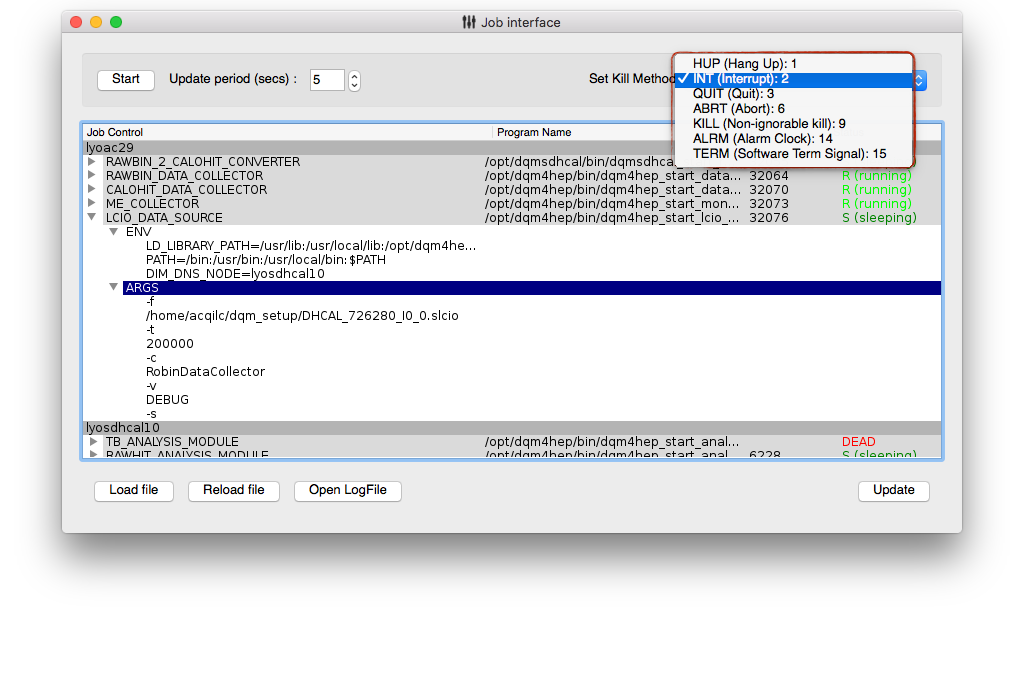
\includegraphics[width=0.7\textwidth]{figs/JobInterface/JobInterface_KillSwitch.png}\end{onlyenv}
       		\begin{onlyenv}<2>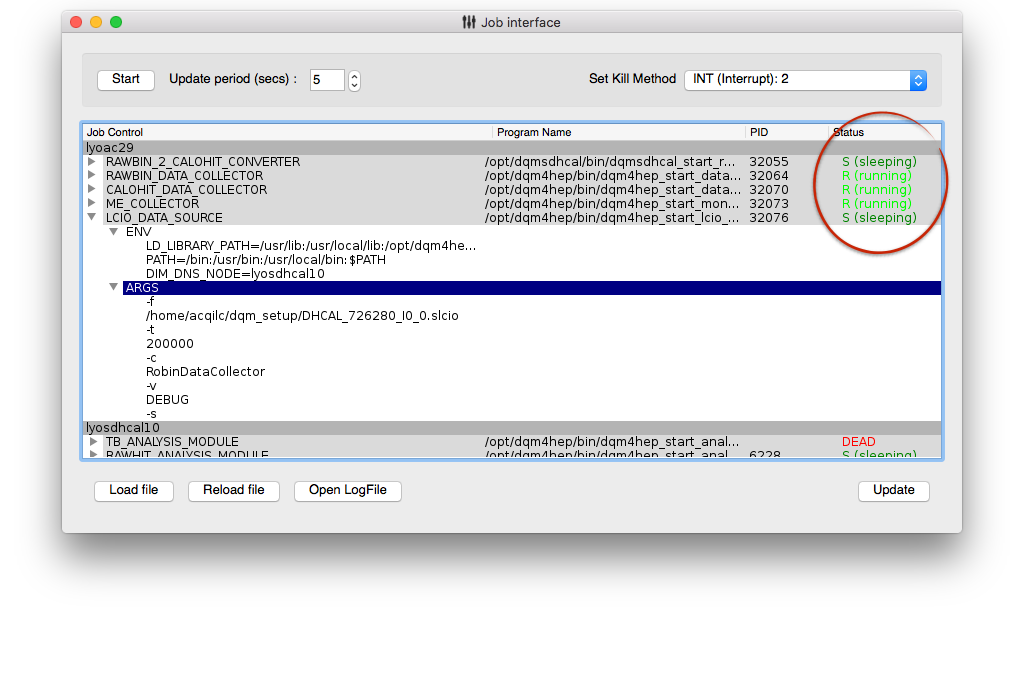
\includegraphics[width=0.7\textwidth]{figs/JobInterface/JobInterface_LiveStatus.png}\end{onlyenv}
        		\begin{onlyenv}<4>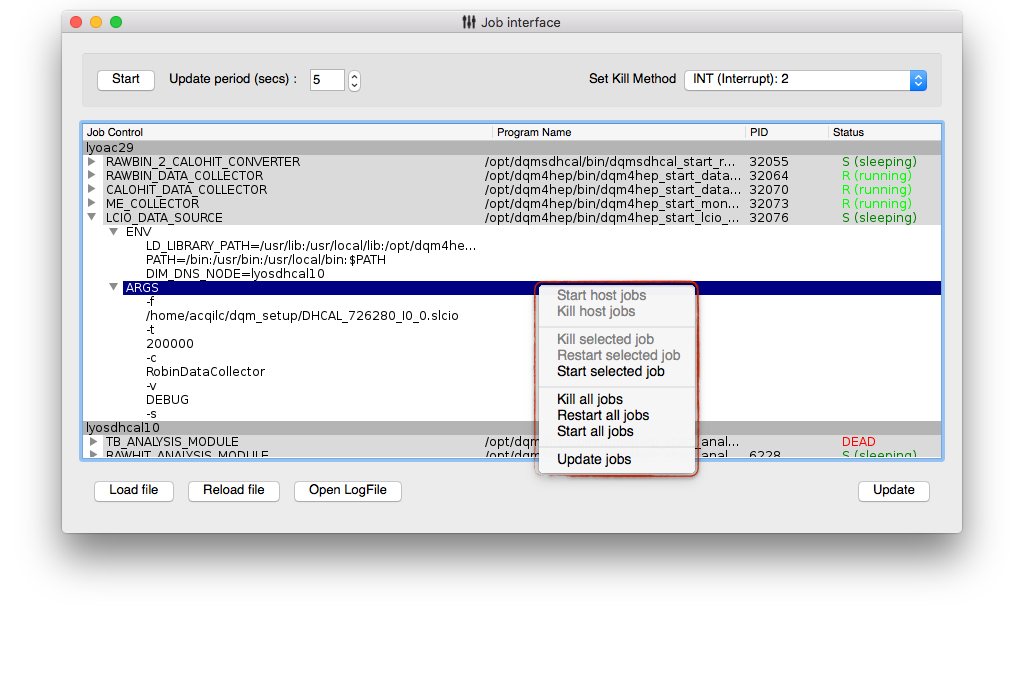
\includegraphics[width=0.7\textwidth]{figs/JobInterface/JobInterface_Module.png}\end{onlyenv}
        		\begin{onlyenv}<1>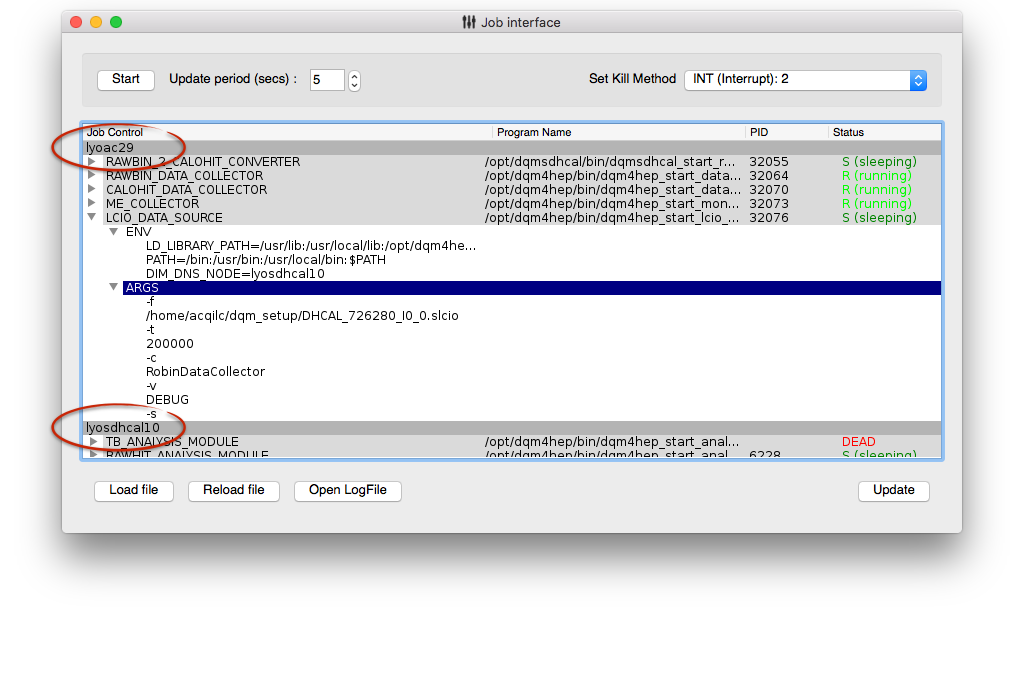
\includegraphics[width=0.7\textwidth]{figs/JobInterface/JobInterface_MultiHost.png}\end{onlyenv}
        		\begin{onlyenv}<3>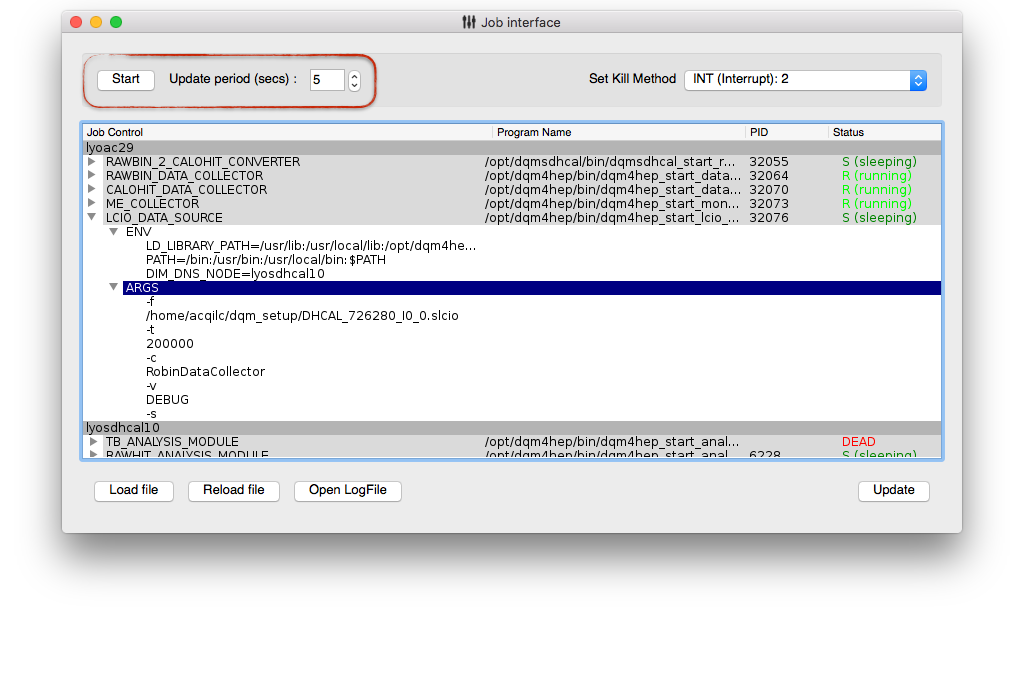
\includegraphics[width=0.7\textwidth]{figs/JobInterface/JobInterface_Update.png}\end{onlyenv}
        		%\begin{onlyenv}<6>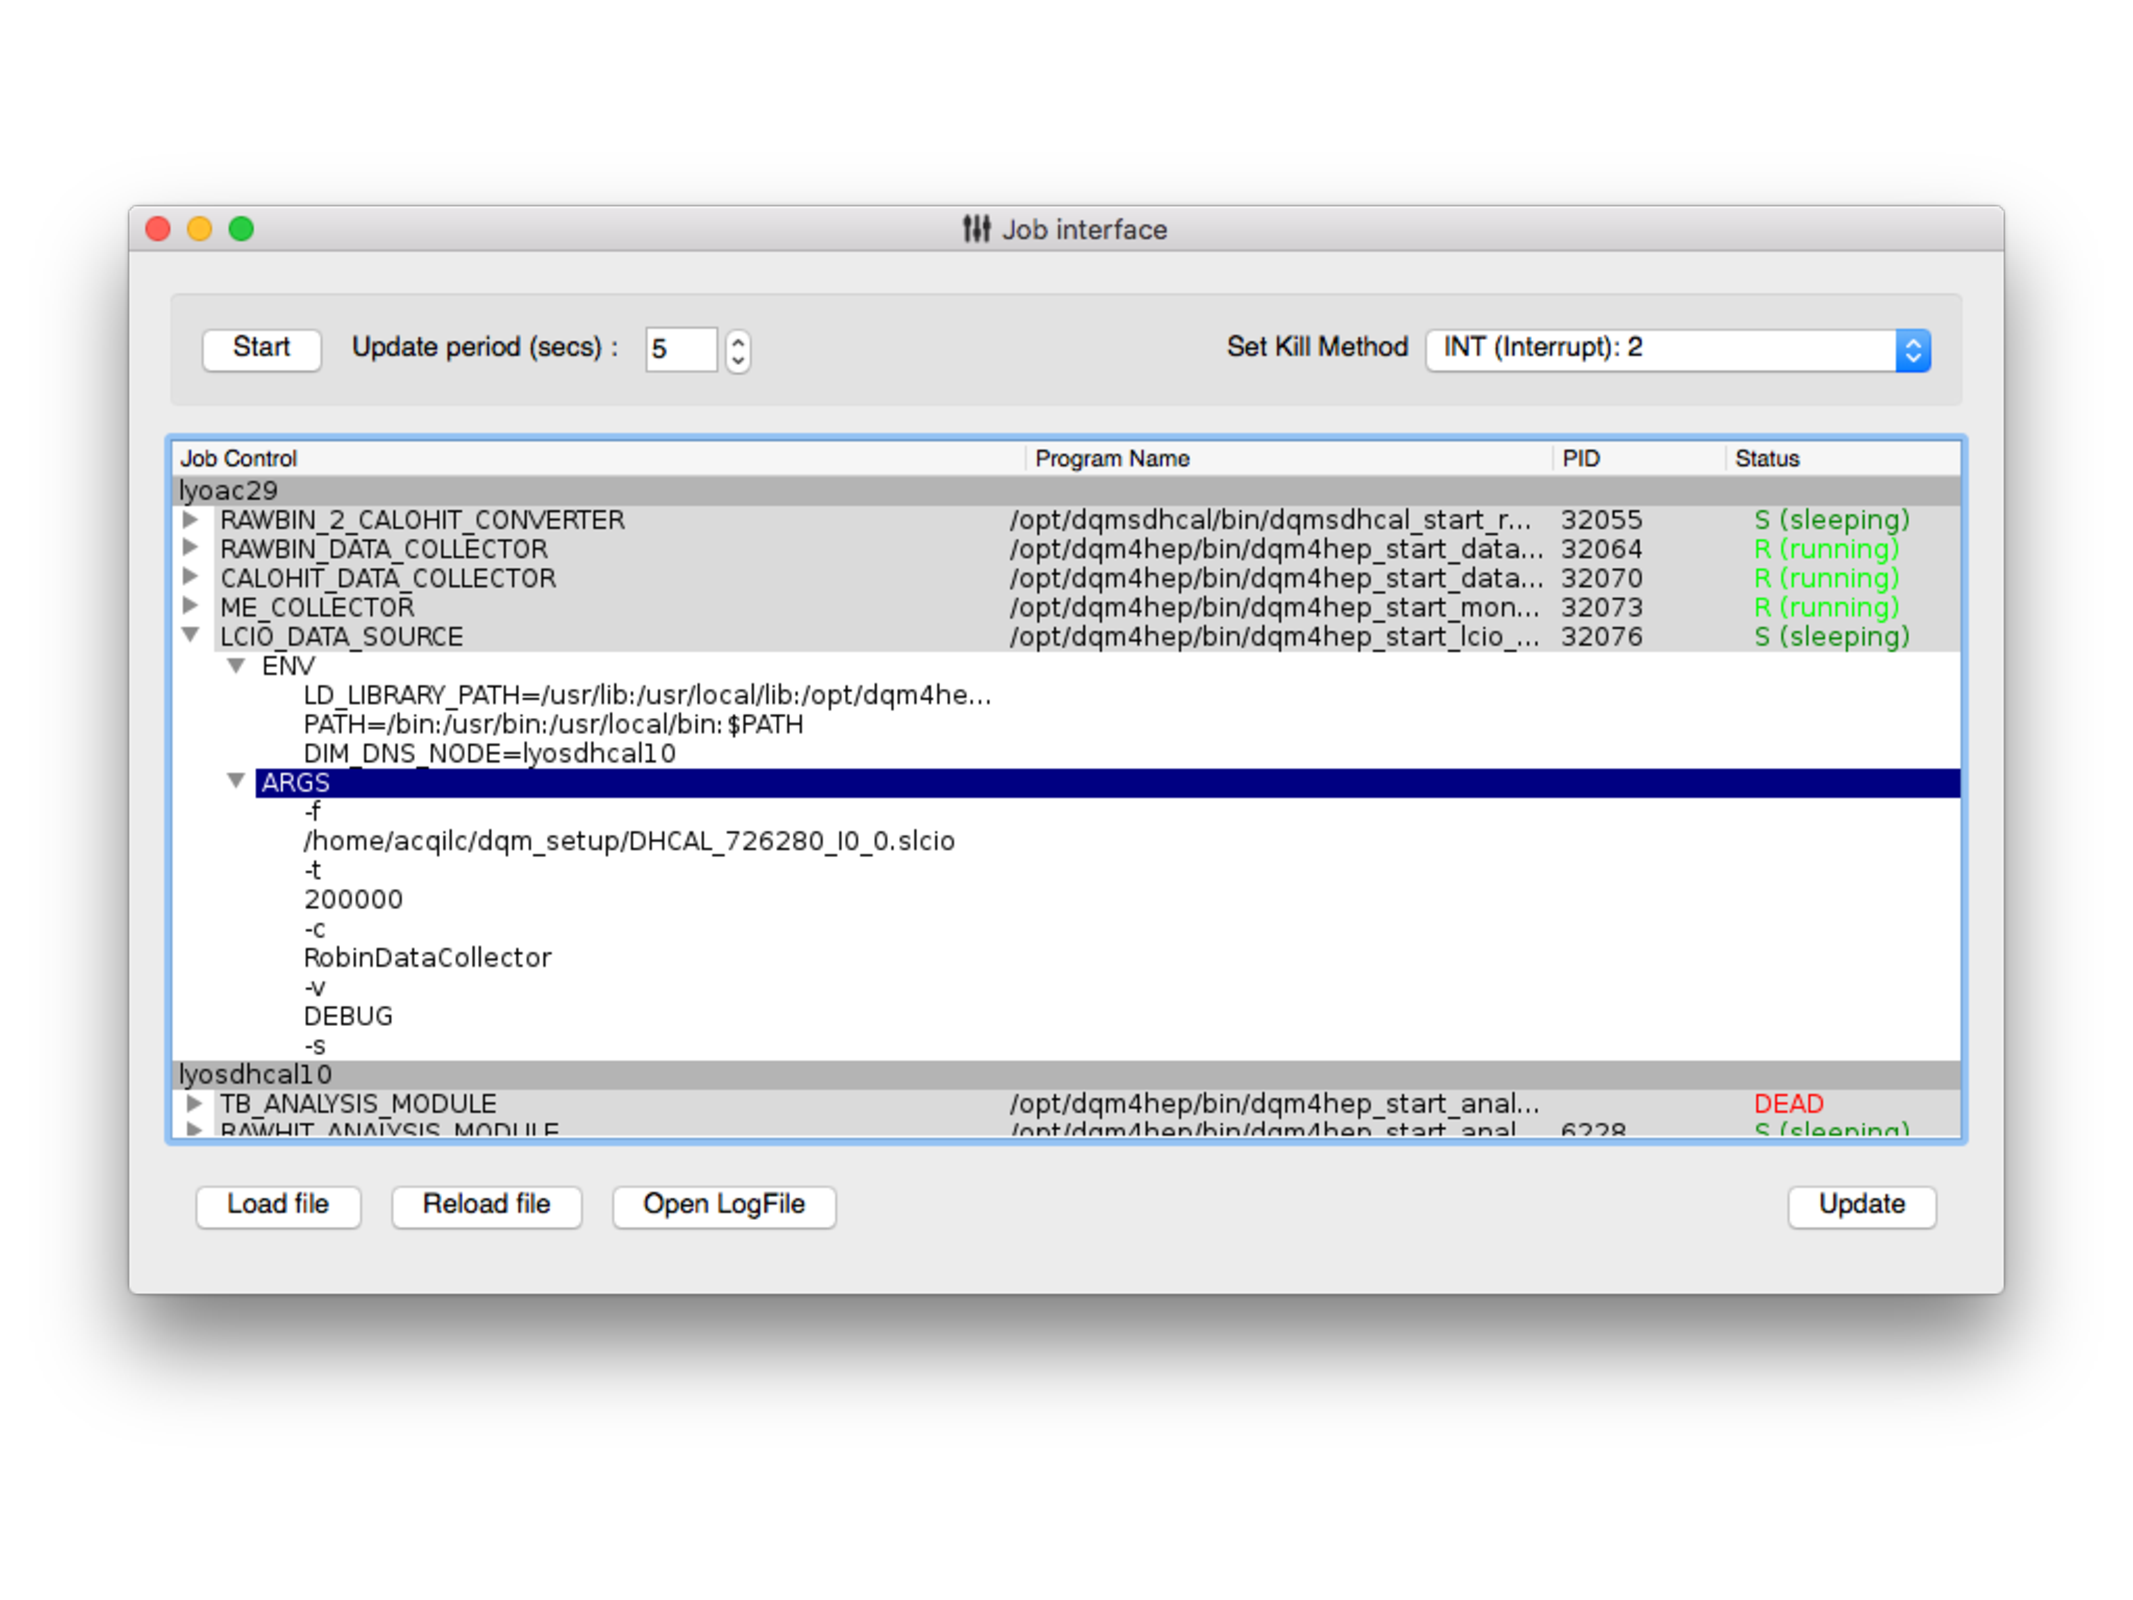
\includegraphics[width=0.7\textwidth]{figs/JobInterface.pdf}\end{onlyenv}	
      \end{center}
      \vspace{-5em}
       \begin{minipage}{\textwidth}

        \begin{itemize}
          \uncover<1->{ \item Load and display a list of applications (Collectors, Modules, etc.) available on different hosts }
       	  \uncover<2->{ \item Displays informations(Name, Host, PID, Status, etc.) about applications }
	        \uncover<3->{ \item Infos can be updated in "real time"}
       	  \uncover<4->{\item Manage Applications (Start/Kill/Restart) with contextual menu }
       	  \uncover<5->{\item Kill method can be adjusted }
       	  %\uncover<6->{\item Query and display log file contents }
      \end{itemize}

    \end{minipage}


    \end{overlayarea}
  \end{frame}


   %% Monitoring Control %%
   %% Browser %%
 \begin{frame}
    \frametitle{\secname}
    \framesubtitle{ Monitoring Gui + Browser }

    \begin{overlayarea}{\textwidth}{\textheight}
    	       \begin{center}

        \begin{onlyenv}<1>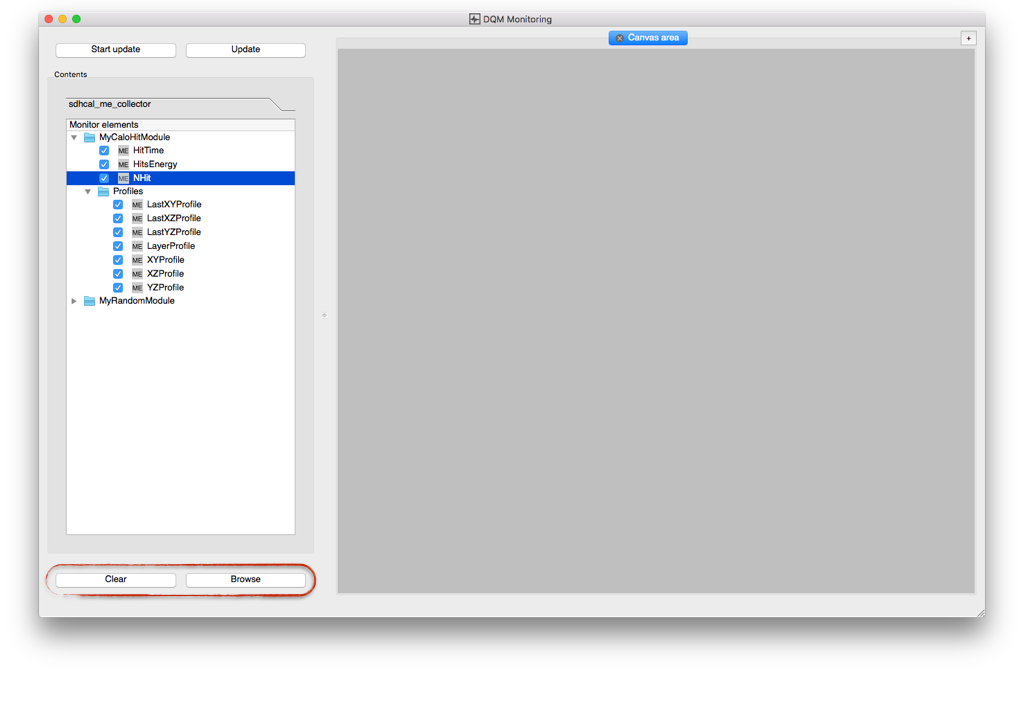
\includegraphics[width=0.8\textwidth]{figs/MonitoringGui/MG_Browse.png}\end{onlyenv}
                       \end{center}

       \begin{columns}

	 \column{.55\textwidth}
	 \vspace{-3em}

	\begin{center}
%          \begin{onlyenv}<2>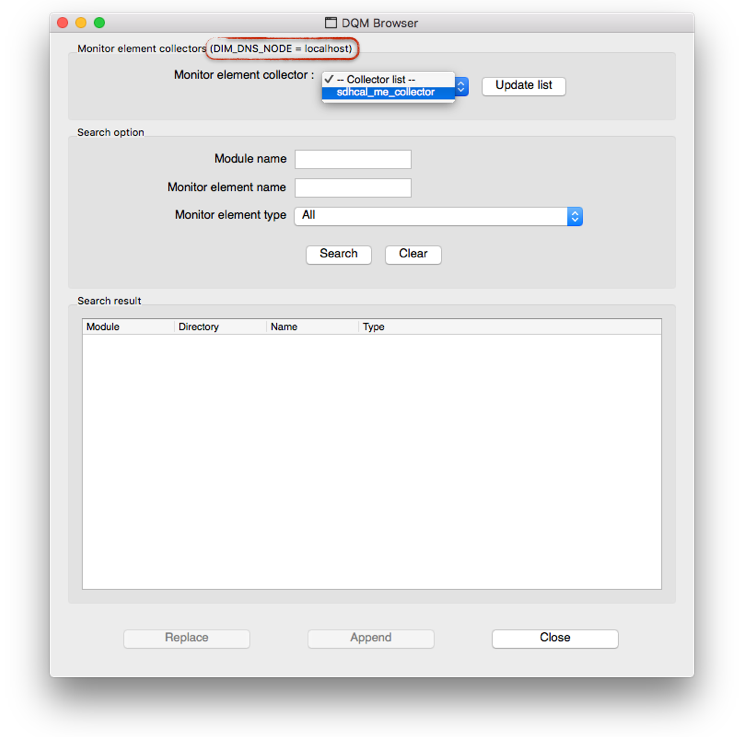
\includegraphics[width=1.1\textwidth]{figs/Browser/Browser_DNSNode.png}\end{onlyenv}
%          \begin{onlyenv}<3>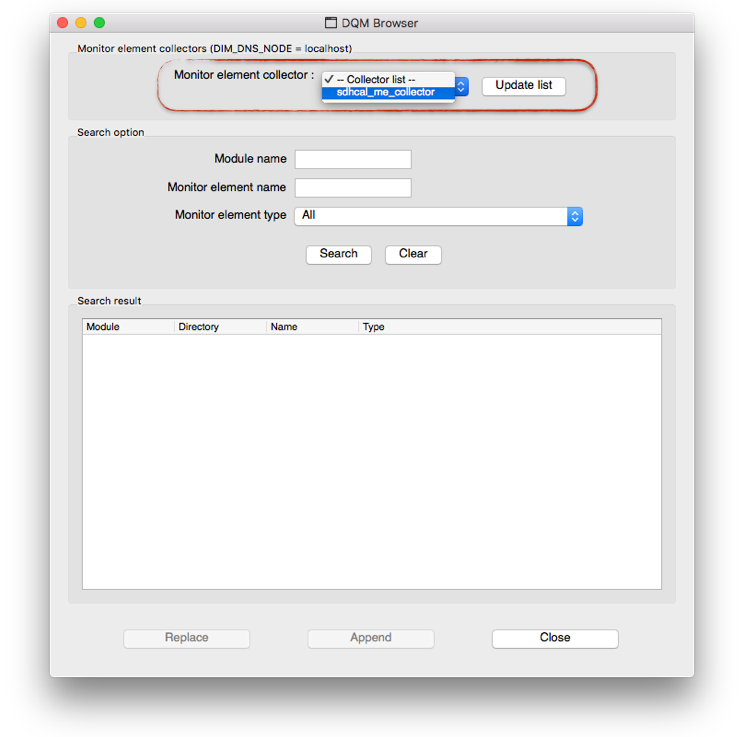
\includegraphics[width=1.1\textwidth]{figs/Browser/Browser_MESelection}\end{onlyenv}
%          \begin{onlyenv}<4>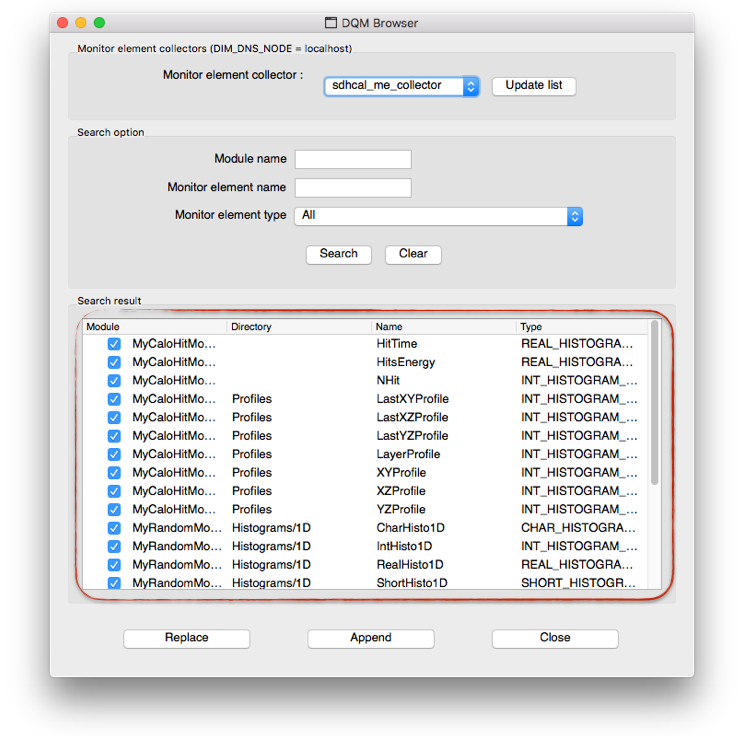
\includegraphics[width=1.1\textwidth]{figs/Browser/Browser_FullList}\end{onlyenv}
%          \begin{onlyenv}<5>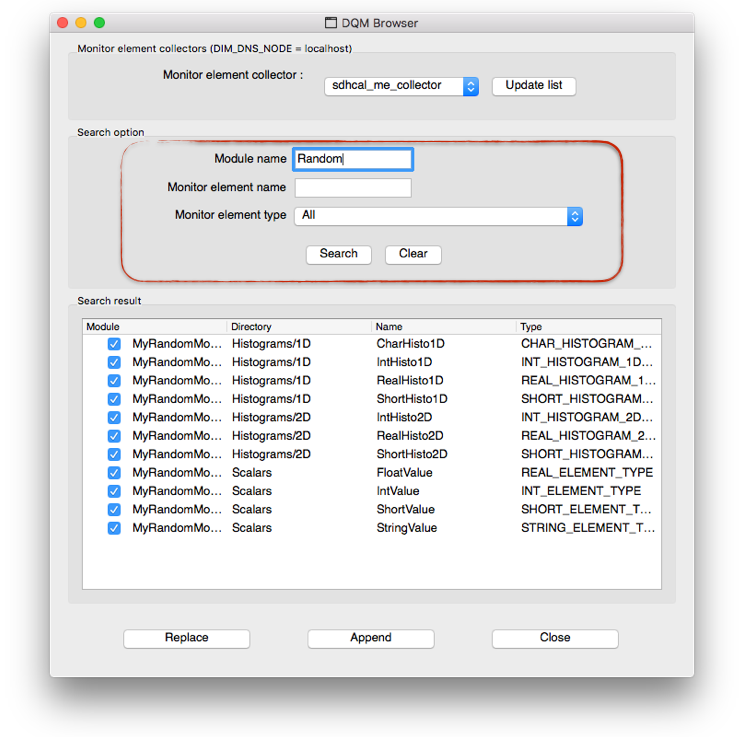
\includegraphics[width=1.1\textwidth]{figs/Browser/Browser_Search}\end{onlyenv}
         \begin{onlyenv}<2>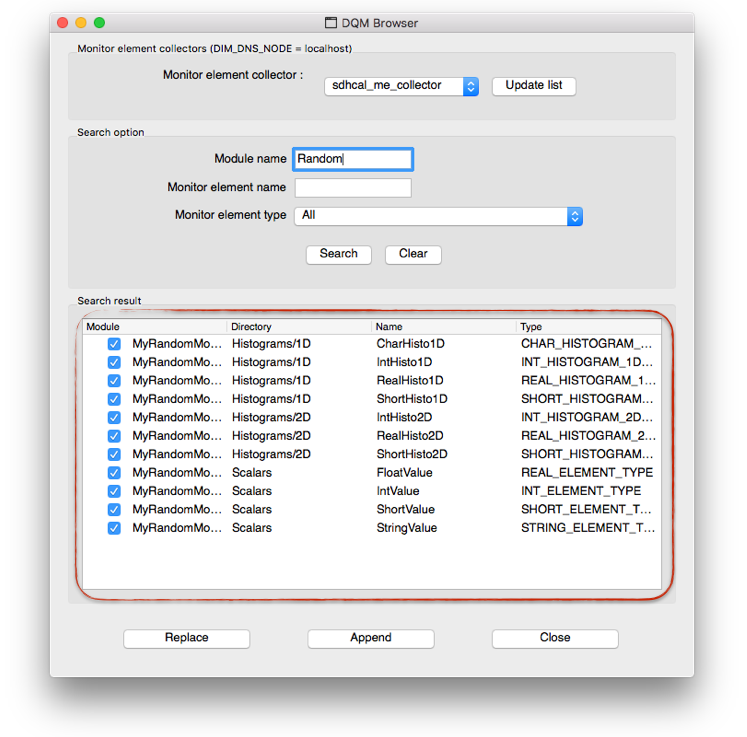
\includegraphics[width=1.1\textwidth]{figs/Browser/Browser_SearchResult}\end{onlyenv}
               \end{center}

         \column{.45\textwidth}
         \begin{itemize}
         \uncover<2->{ \item Browser to build histograms selections to display }
       	 \uncover<2->{\item Search Function to refine selection }
      \end{itemize}

           \end{columns}
               \end{overlayarea}

  \end{frame}


  %% Control Gui %%
  \begin{frame}
    \frametitle{\secname}
    \framesubtitle{ Monitoring Gui + Browser }
    \begin{overlayarea}{\textwidth}{\textheight}
    \vspace {-1em}
      \begin{center}
         \begin{onlyenv}<1>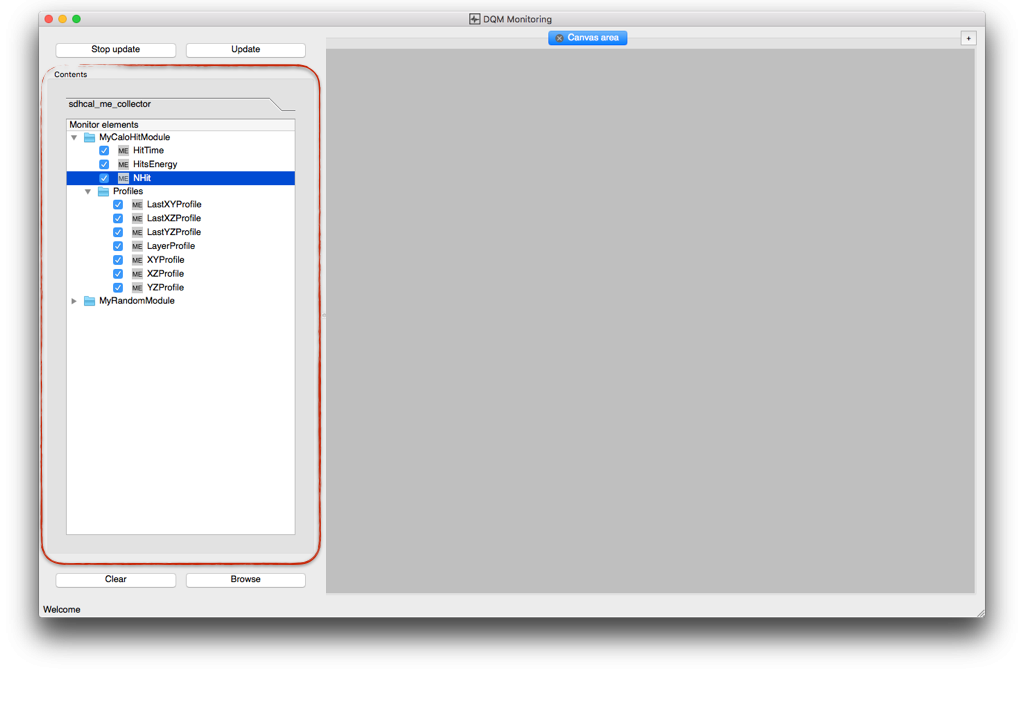
\includegraphics[width=0.8\textwidth]{figs/MonitoringGui/MG_Content}\end{onlyenv}
         \begin{onlyenv}<2>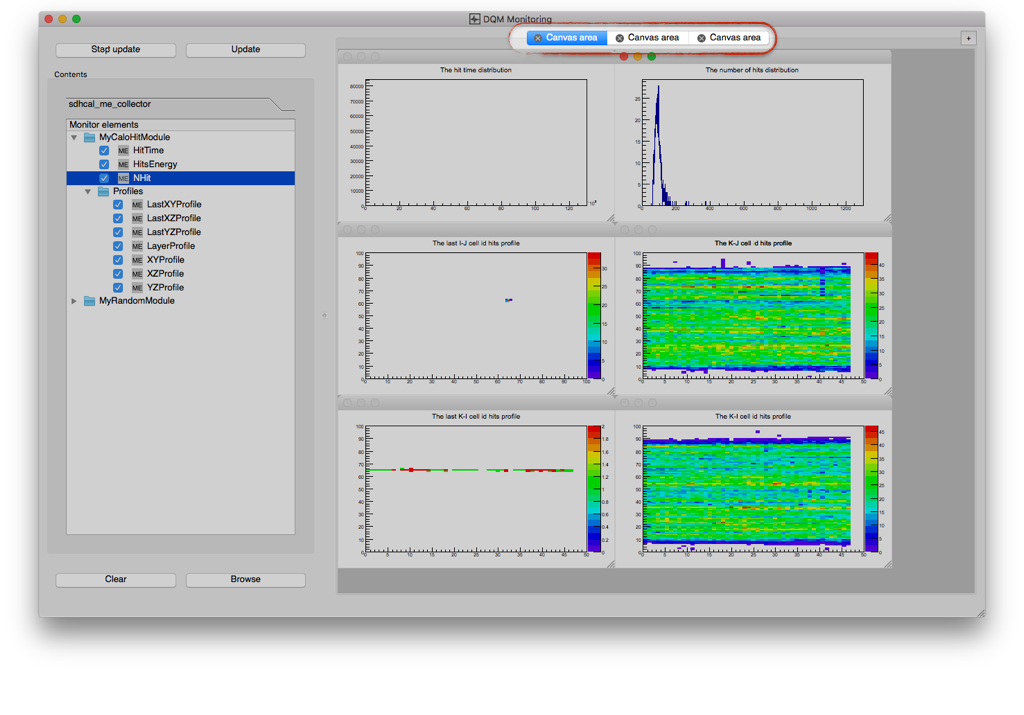
\includegraphics[width=0.8\textwidth]{figs/MonitoringGui/MG_Tabs}\end{onlyenv}
         \begin{onlyenv}<3>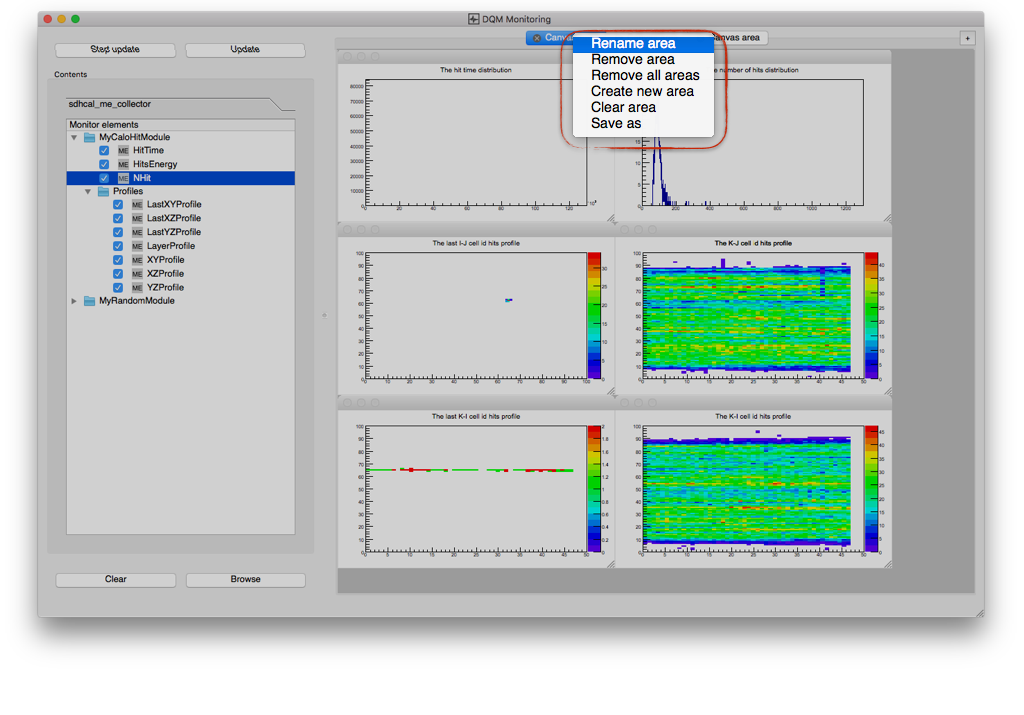
\includegraphics[width=0.8\textwidth]{figs/MonitoringGui/MG_TabsMenu}\end{onlyenv}
         \begin{onlyenv}<4>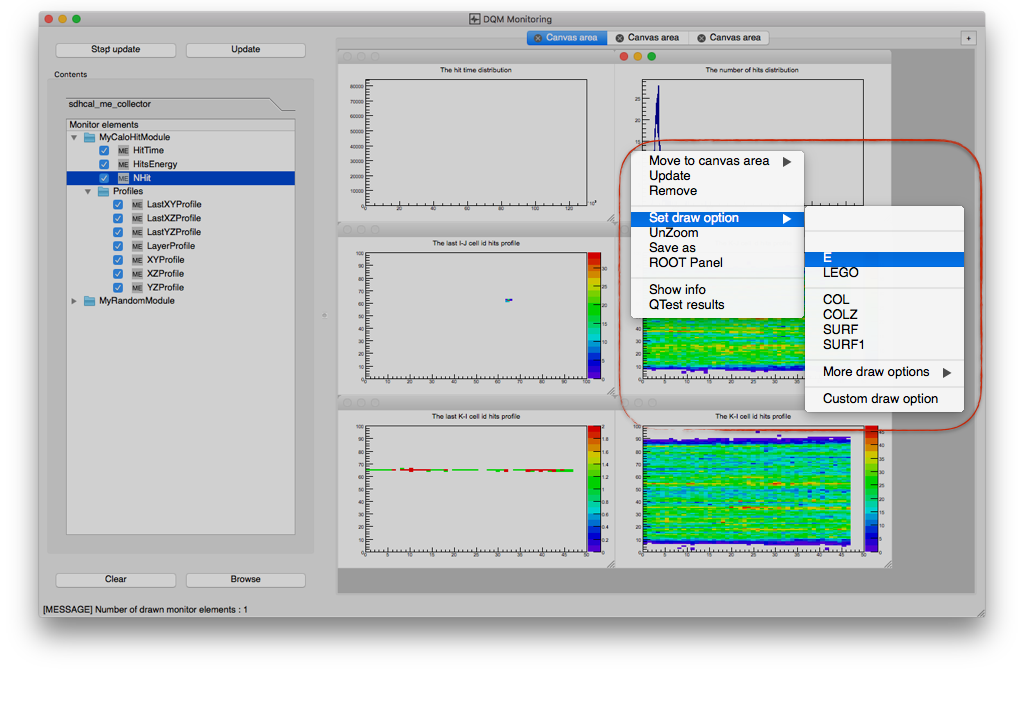
\includegraphics[width=0.8\textwidth]{figs/MonitoringGui/MG_HistosMenu}\end{onlyenv}
         \begin{onlyenv}<5>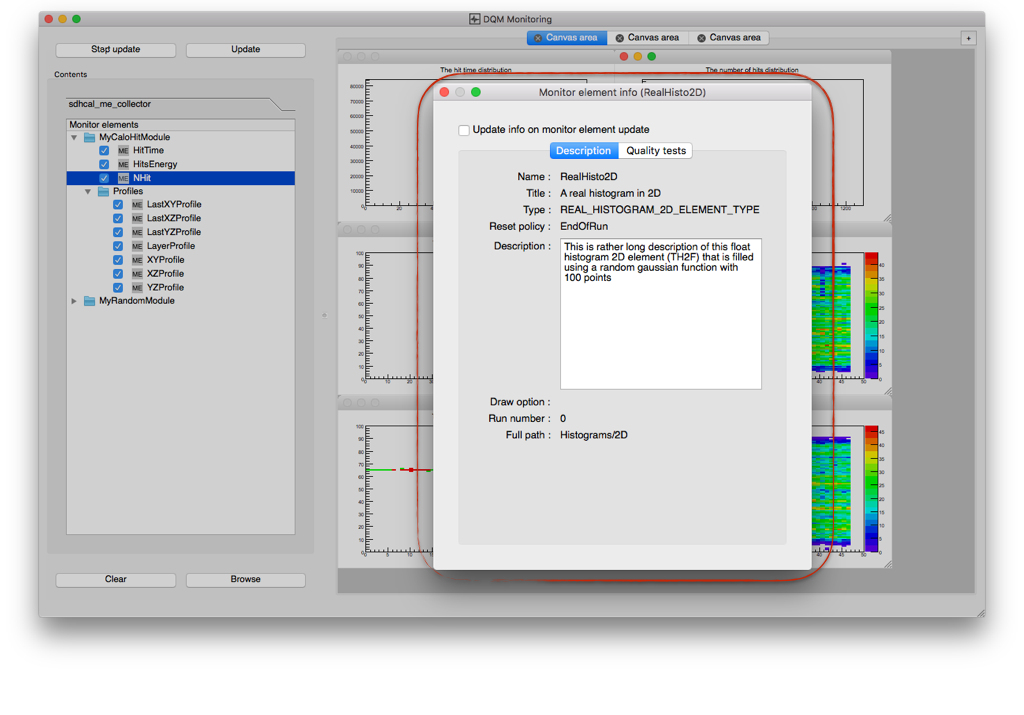
\includegraphics[width=0.8\textwidth]{figs/MonitoringGui/MG_HistoInfo}\end{onlyenv}
         \begin{onlyenv}<6>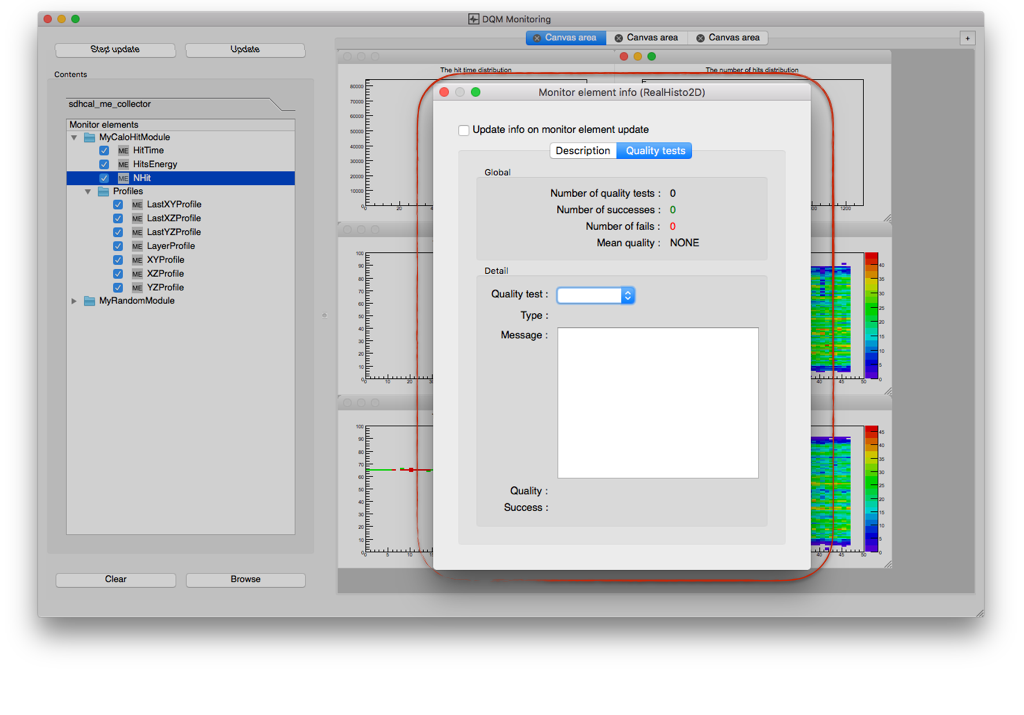
\includegraphics[width=0.8\textwidth]{figs/MonitoringGui/MG_HistoQuality}\end{onlyenv}
         \begin{onlyenv}<7>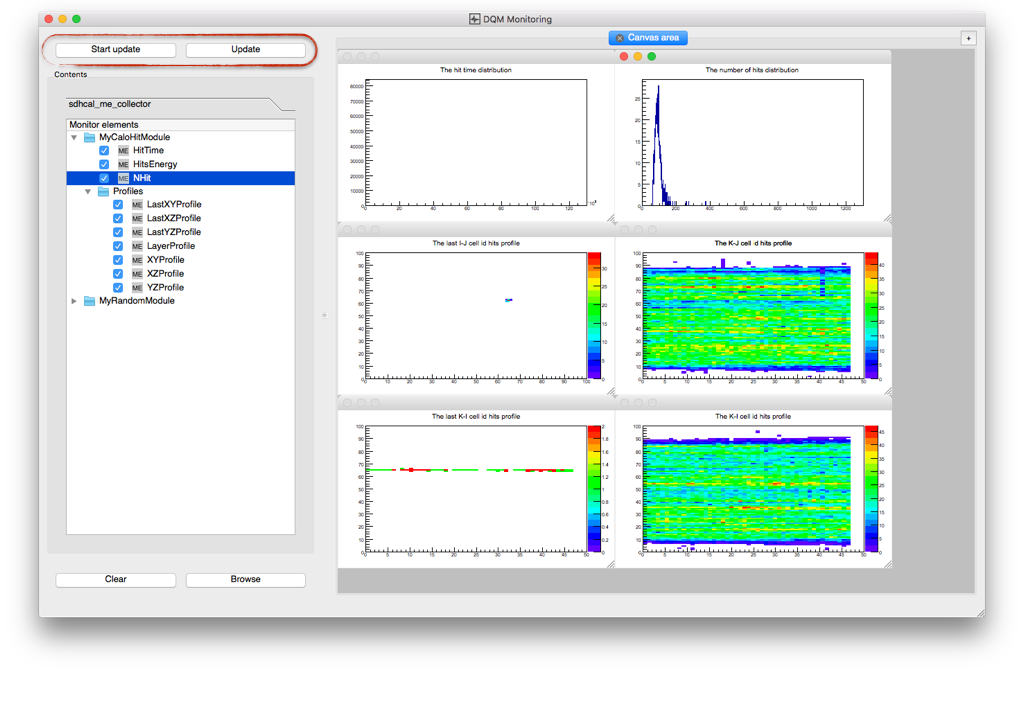
\includegraphics[width=0.8\textwidth]{figs/MonitoringGui/MG_AutoUpdate.png}\end{onlyenv}
      \end{center}
      \vspace{-3em}
      \begin{minipage}{\textwidth}
        \begin{itemize}
          \uncover<1-1>{ \item List of histograms added from Browser }
          \vspace{-1.5em}
       	  \uncover<2->{ \item Multiple canvas area available}
       	  \uncover<4->{ \item Real ROOT histograms (Can be fitted, zoomed, etc.) }
       	  \uncover<5-6>{\item Histograms descriptions and Quality}
       	  \vspace{-1.5em}
       	  \uncover<7->{\item Auto Update }
        \end{itemize}
      \end{minipage}
    \end{overlayarea}
  \end{frame}
  
  \section{DQM for SDHCAL prototype}
  
  \begin{frame}
    \frametitle{\secname}
    Implements online analysis for the SDHCAL $m^3$ prototype. \\
    ~ \\
    Development made in parallel with the DQM4HEP framework \\
    Use last DQM4HEP version (currently v04-03-00) \\
    ~ \\
    Additional software used : 
    \begin{itemize}
      \item \textbf{Trivent} : standalone and generic time clustering.
      \item \textbf{CaloSoftWare} : various SDHCAL analysis tools from A. Steen :
      \begin{itemize}
        \item Calo Hit clustering
        \item Global and local (Hough) tracking
        \item Interaction finder
        \item Tools for efficiency/multiplicity estimate
      \end{itemize}
    \end{itemize}
    ~ \\
    The DQM for SDHCAL provides :
    \begin{itemize}
      \item Analysis tools for online data treatment
      \item Data conversions (raw buffer -> raw calo hit -> calo hit)
      \item Shm processors to SDHCAL DAQ
      \item Set of DQM modules
    \end{itemize}
  \end{frame}
  
  
  \begin{frame}
    \frametitle{\secname}
    \framesubtitle{SDHCAL analysis tools}
    \begin{block}{Online data feeding}
    Implementation of shm plugin (levbdim) with LCEvent data structure :
      \begin{itemize}
        \item Event info : fill LCEvent information
        \item SDHCAL RawCalorimeterHit collection creation : from DIFs raw buffer to hits
        \item Cherenkov RawCalorimeterHit collection creation : from BIF (generally DIF id=3) to cherenkov hits
      \end{itemize}
    \end{block}
    ~ \\
    Send LCEvent to event collector ! \\
    ~ \\
    \underline{Missing} : SiWECAL shm plugin. Which raw data structure ? \\
    Need conversion to RawCalorimeterHit format (cellID + energy + time stamp)
  \end{frame}
  
  
  
  \begin{frame}[containsverbatim]
    \frametitle{\secname}
    \framesubtitle{Online builder - SDHCAL implementation}
    \begin{center}
      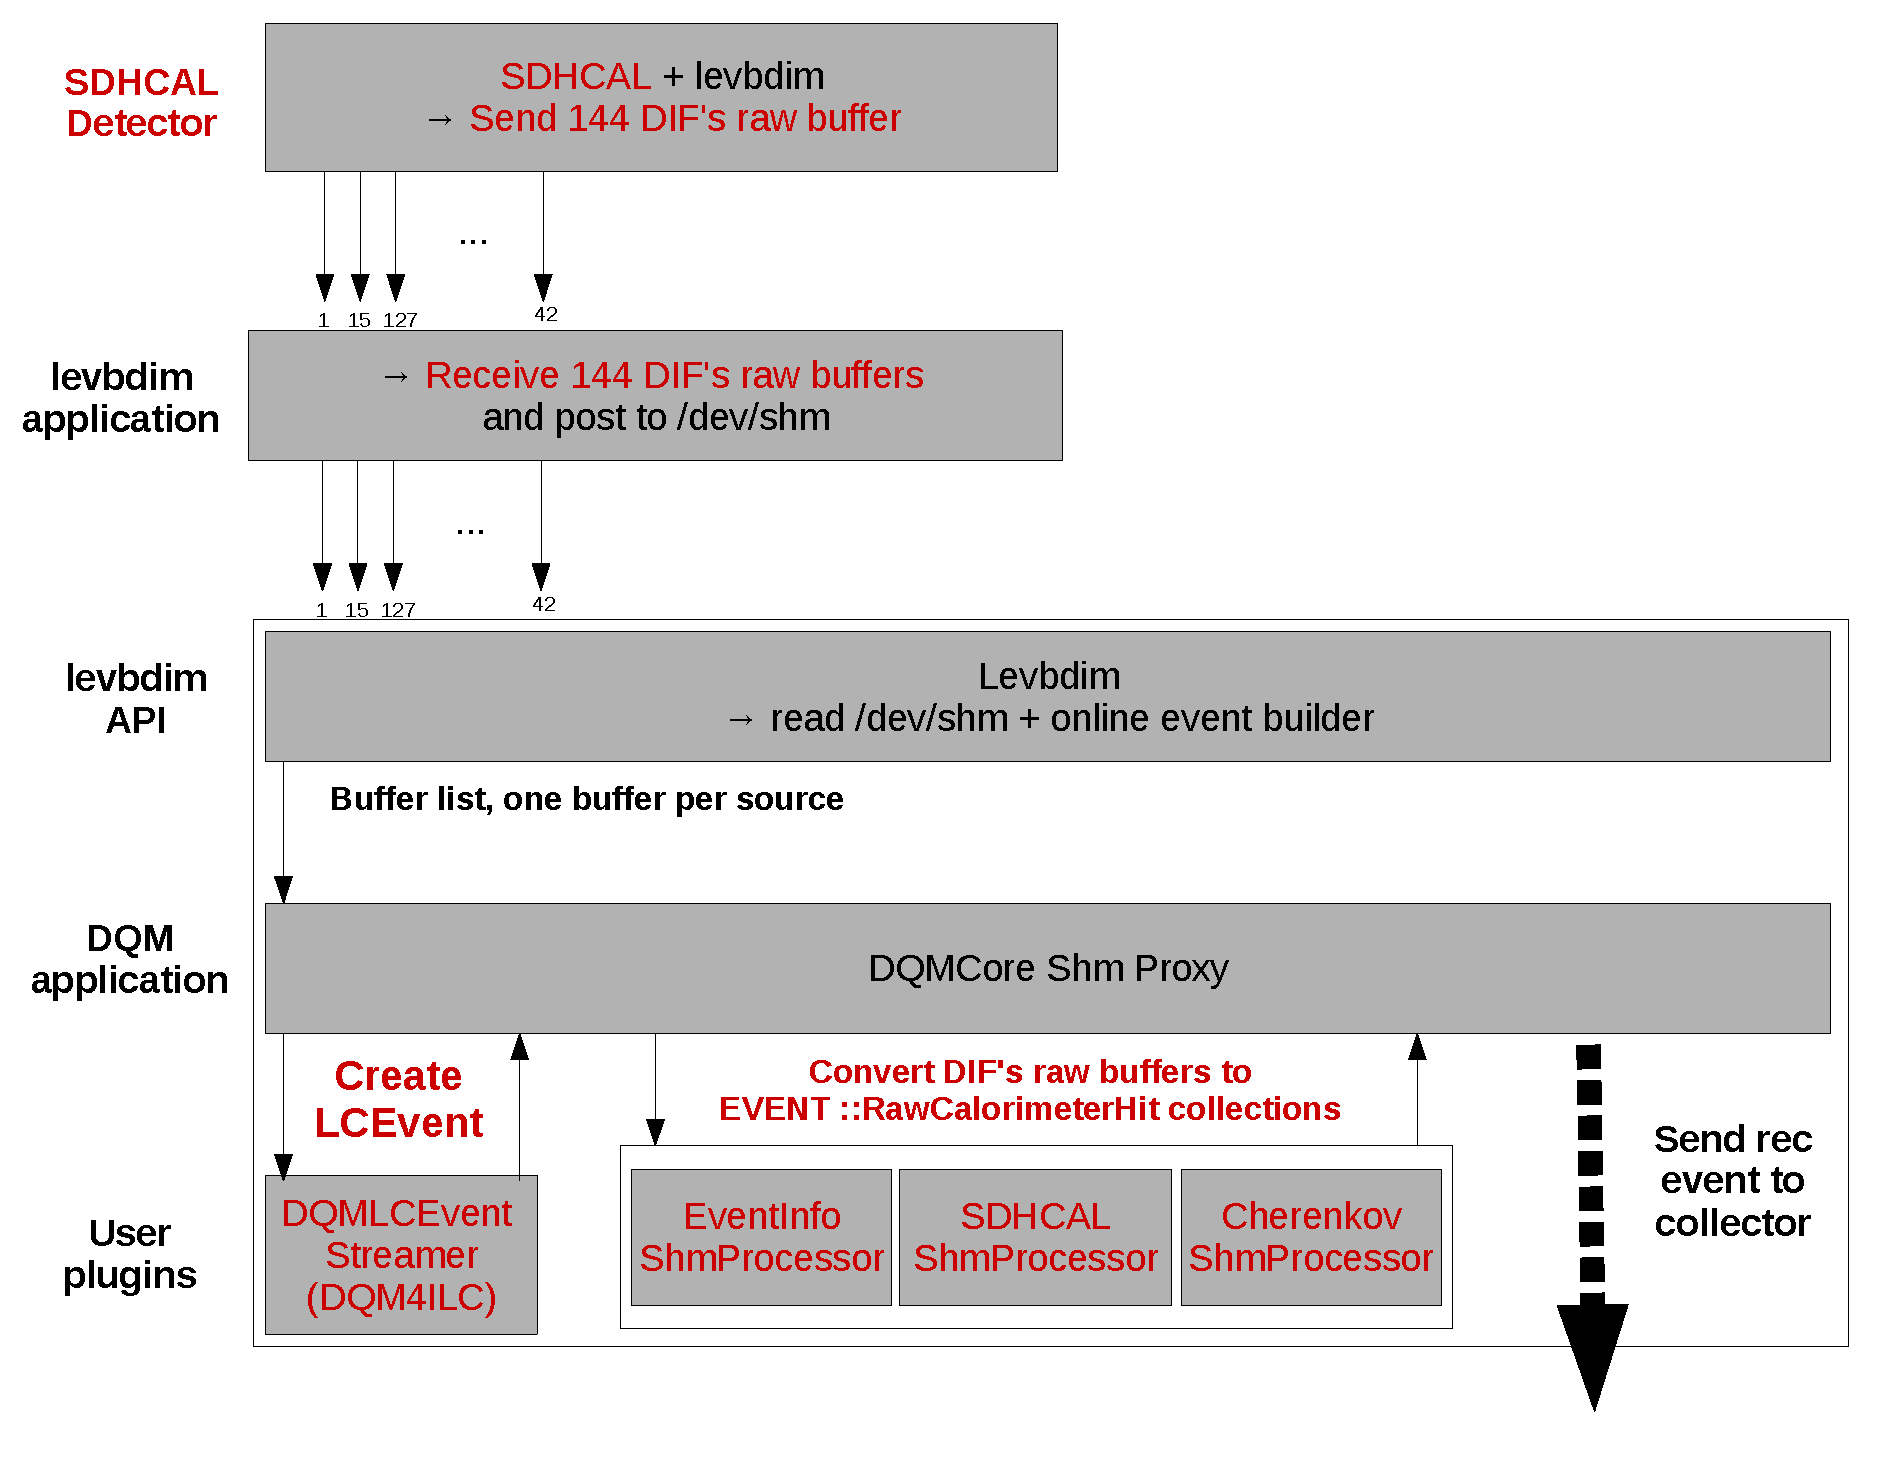
\includegraphics[width=0.8\textwidth]{figs/DQMeventbuilder_sdhcal.pdf}
    \end{center}
  \end{frame}
  
  
  \begin{frame}[containsverbatim]
    \frametitle{\secname}
    \framesubtitle{SDHCAL analysis tools}
    \begin{block}{Event classifier}
      Class \verb|EventClassifier| from DQMSDHCAL package\\ ~\\
      Interface to particle ID for online analysis. User needs to implements \verb|processEvent(LCEvent*)| and decide for one of the following tag : \\ 
      ~ \\
      {\tt Undefined, noise event, beam muon, cosmic muon, charged/neutral em shower, charged/neutral had shower} \\
      ~ \\
      
      Various analysis in SDHCAL DQM modules uses this plugin to perform particle id dependent analysis. \\
      SDHCAL Event classifier implemented. \\~\\
      \underline{Missing} : SiWECAL + SDHCAL event classifier. In particular, electrons will be stopped before entering the SDHCAL -> different identification
    \end{block}
  \end{frame}
    
    
  \begin{frame}[containsverbatim]
    \frametitle{\secname}
    \frametitle{SDHCAL analysis tools}
    \begin{block}{Electronics mapping}
      Class \verb|DQMElectronicsMapping| from DQMCore package \\~\\
      Transparent conversion of (DIF id, Asic id, Channel ID) $\leftrightarrow$ (I, J, layer) $\leftrightarrow$ (x, y, z) \\
      SDHCAL electronics mapping implemented (with Hardroc2). \\~\\
      \underline{Missing} : SiWECAL electronics mapping
    \end{block}
    \begin{block}{LCCollection converters}
      Class \verb|DQMDataConverter<LCCollection, LCCollection>| from DQMCore package \\~\\
      Transparent conversion from one collection to another. \\
      SDHCAL data convert implemented. Converts RawCalorimeterHit collection (DIF, Asic, Channel) to CalorimeterHit collection (x, y, z) \\~\\
      \underline{Missing} : SiWECAL data conversion (same io types) \\
    \end{block}
  \end{frame}
  
  
  \begin{frame}[containsverbatim]
    \frametitle{\secname}
    \framesubtitle{SDHCAL analysis tools}
    \begin{block}{Trivent module}
      Class \verb|DQMAnalysisModule| from DQMCore package and \verb|LCTriventListener| from Trivent package\\~\\
      \verb|DQMTriventModule| is a base class that runs Trivent on \textit{trigger} event $\rightarrow$ split the input event into \textit{time clustered} event representing each a particle event. \\~\\
      Global idea :
      \begin{itemize}
        \item Fill Trivent with input collections
        \item Run Trivent
        \item For each clustered event : convert each LCCollection using data converter plugins and notify user that a physics event has been reconstructed
      \end{itemize}
      ~ \\
      In DQMSDHCAL, most of the analysis modules inherits this module to analyze directly particle per particle events 
    \end{block}
  \end{frame}
  
  \section{SDHCAL modules}
  
  
  
  \begin{frame}[containsverbatim]
    \frametitle{\secname}
    \framesubtitle{\textit{AsicAnalysisModule}}
    \begin{block}{Purpose}
      Inherits from \verb|DQMTriventModule| and analyze particle per particle events. \\
      Use CaloSoftWare to find and analyze muons (beam and cosmic ones) in detector. \\
      Can be adapted to SiWECal by tunning some parameters in xml only
    \end{block}
    
    \begin{block}{Monitor elements}
      \begin{itemize}
        \item Layer efficiency (thr 1,2,3) (TH1)
        \item Layer multiplicity (TH1)
        \item Per layer :
        \begin{itemize}
          \item Asic efficiency map (thr 1,2,3) (TH2)
          \item Asic multiplicity map (TH2)
        \end{itemize}
        \item Asic efficiency (thr 1,2,3) (TH1)
        \item Asic multiplicity (TH1)
        \item Asic stacked efficiency map (thr 1,2,3) (TH2)
        \item Asic stacked multiplicity (TH2)
        \item N track per asic (TH1)
      \end{itemize}      
    \end{block}
  \end{frame}
  
  
  
  
  \begin{frame}[containsverbatim]
    \frametitle{\secname}
    \framesubtitle{Conclusion and questions}
    \begin{block}{Conclusion}
      \begin{itemize}
        \item Online DQM for SDHCAL developed using DQM4HEP
        \item Finalizing monitoring depending on your remarks
        \item Need SiWECal implementation for upcoming beam test in June.
      \end{itemize}
    \end{block}
    \begin{block}{Needs from SiWECal team}
      \begin{itemize}
        \item Electronics mapping. Geometry conversion of (DIF, Roc, Channel) $\leftrightarrow$ (I, J, layer) $\leftrightarrow$ (x,y,z)
        \item Data conversion :
        \begin{itemize}
          \item from raw data from each DIF (ECAL format) to RawCalorimeterHit collection (DIF, Roc, Channel, time, energy)
          \item from RawCalorimeterHit to CalorimeterHit using electronics mapping
        \end{itemize}
        \item Shm processor using the raw data conversion
        \item Common analysis tools :
        \begin{itemize}
          \item Combined particle ID functions
        \end{itemize}
      \end{itemize}
      ~ \\
      If you want to see more things implemented in the DQM system for the ECal, let us know !
      
    \end{block}
  \end{frame}
  

\end{document}
